\chapter{ORGANIZAÇÃO CURRICULAR}

Levando em consideração as orientações contidas na Resolução CNE/CES num. 5 de 11/2016, que institui as Diretrizes Curriculares Nacionais para os cursos de graduação na área da Computação, o currículo do curso de Bacharelado em Ciência da Computação apresenta a seguinte estrutura conforme Quadro 3 abaixo:

\begin{center}
  \begin{scriptsize}
    \begin{longtable}{@{}lp{10cm}}
      \caption{\label{quadro:organizacao-curricular-do-curso}Organização curricular do curso.}\\
    \toprule
    \textbf{Núcleo de Conhecimento} & \textbf{Componentes Curriculares} \\ 
    \midrule
    Conteúdos Básicos & PRÉ-CÁLCULO\\ 
                      & LÓGICA MATEMÁTICA \\
                      & COMPUTADORES E SOCIEDADE \\
                      & INGLÊS  \\
                      & CÁLCULO I \\
                      & GEOMETRIA ANALÍTICA \\
                      & METODOLOGIA CIENTÍFICA \\
                      & INGLÊS INSTRUMENTAL \\
                      & CÁLCULO II \\
                      & ÁLGEBRA LINEAR I \\
                      & MATEMÁTICA DISCRETA PARA COMPUTAÇÃO \\
                      & PROBABILIDADE E ESTATÍSTICA \\
                      & FÍSICA PARA COMPUTAÇÃO \\ \midrule
    Conteúdos Tecnológicos  & INTRODUÇÃO À CIÊNCIA DA COMPUTAÇÃO \\ 
                            & INTRODUÇÃO À PROGRAMAÇÃO \\
                            & ALGORITMOS E ESTRUTURA DE DADOS II \\
                            & PROGRAMAÇÃO ORIENTADA A OBJETOS \\
                            & ALGORITMOS E ESTRUTURA DE DADOS \\
                            & SISTEMAS DIGITAIS \\
                            & PARADIGMAS DE LINGUAGENS DE PROGRAMAÇÃO \\
                            & INTERAÇÃO HUMANO COMPUTADOR \\
                            & BANCO DE DADOS \\
                            & INTELIGÊNCIA ARTIFICIAL \\
                            & ARQUITETURA DE COMPUTADORES \\
                            & PROJETO E ANÁLISE DE ALGORITMOS \\
                            & REDES DE COMPUTADORES \\
                            & SISTEMAS OPERACIONAIS \\
                            & TEORIA DA COMPUTAÇÃO \\
                            & COMPUTAÇÃO GRÁFICA \\
                            & ENGENHARIA DE SOFTWARE \\
                            & SISTEMAS DISTRIBUÍDOS \\
                            & EMPREENDIMENTOS EM TIC \\
                            & PROJETO DE DESENVOLVIMENTO DE SOFTWARE \\
                            & PROGRAMAÇÃO WEB \\
                            & SISTEMAS DE INFORMAÇÃO E TECNOLOGIAS \\
                            & APRENDIZAGEM DE MÁQUINA \\
                            & PROCESSAMENTO DIGITAL DE IMAGENS \\
                            & COMPILADORES \\
                            & ESTÁGIO SUPERVISIONADO OBRIGATÓRIO \\
                            & TRABALHO DE CONCLUSÃO DE CURSO I \\
                            & TRABALHO DE CONCLUSÃO DE CURSO II \\
    \bottomrule
    \end{longtable}
  \end{scriptsize}      
\end{center}

A carga horária total do curso de Bacharelado em Ciência da Computação tem um total de 3.200h horas, sendo distribuída em 4,5 (quatro vírgula cinco) anos, isto é, 9 (nove) períodos. Os conteúdos de formação serão apresentados em componentes curriculares com carga horária variando entre 30h e 60h para as disciplinas, 300h para ESO e para TCC 1 60h e TCC 2 180h. Cada hora-aula corresponde a 60 minutos, conforme expresso na Resolução CEPE/UFRPE nº 220/2016 e demonstrado no Quadro 4 abaixo.

\begin{center}
  
  \begin{scriptsize}
    \begin{longtable}{p{4cm}p{1.5cm}p{2cm}p{3cm}}
      \caption{\label{quadro:distribuicao-nucleos-formacao-e-ch}Distribuição dos núcleos de formação e carga horária.}\\
    \toprule
    \multicolumn{4}{c}{\textbf{Bacharelado em Ciência da Computação}}\\ \midrule
    \multicolumn{2}{l}{\textbf{Núcleo}} & \multicolumn{1}{c}{\textbf{Carga Horária (h)}} & \multicolumn{1}{c}{\textbf{\%}}\\
    \midrule
    Básicos & & \multicolumn{1}{c}{660} & \multicolumn{1}{r}{20,6}\\ \midrule
    \multirow{3}{3cm}{Tecnológico / Profissionalizante} & Disciplinas & \multicolumn{1}{c}{1.440} & \multicolumn{1}{r}{45,0}\\ \cline{2-4}
    & TCC & \multicolumn{1}{c}{180} & \multicolumn{1}{r}{5,6}\\ \cline{2-4}
    & ESO & \multicolumn{1}{c}{300} & \multicolumn{1}{r}{9,4}\\ \midrule
    \multicolumn{2}{l}{Componentes optativos} & \multicolumn{1}{c}{300} & \multicolumn{1}{r}{9,4}\\ \midrule
    \multicolumn{2}{l}{Atividades complementares} & \multicolumn{1}{c}{320} & \multicolumn{1}{r}{10,0}\\ \midrule
    \multicolumn{2}{l}{Total} & \multicolumn{1}{c}{3.200} & \multicolumn{1}{r}{100,0}\\
\bottomrule
\end{longtable}
\end{scriptsize}      
\end{center}

Para obtenção do título em Bacharel em Ciência da Computação o aluno deverá cumprir uma carga horária total de 3.200h horas, entre disciplinas, atividades complementares, Trabalho de Conclusão de Curso e Estágio Obrigatório Supervisionado. O discente terá a possibilidade de cursar disciplinas do ciclo básico e disciplinas do ciclo tecnológico/profissional, podendo ainda escolher em qual área deseja se aprofundar, uma vez que pode escolher entre as disciplinas optativas que necessita cursar.

As disciplinas de um mesmo período letivo ou de períodos anteriores, no qual o aluno tenha cursado, devem se articular em torno de um ou mais projetos de natureza interdisciplinar, buscando otimizar o processo de avaliação nas disciplinas e uma melhor adequação do esforço para resolução de problemas por parte dos discentes, uma vez que assim eles concentram seus esforços num único projeto que contempla aquelas disciplinas que naturalmente interagem. As disciplinas, em suas atividades e projetos, são baseadas na metodologia de aprendizagem baseada em projetos (\textit{Project Based Learning} (PBL) [Barrows, 1986]). Além do diálogo entre as disciplinas, o curso estará atento à tentativa de promoção de uma educação inclusiva, adaptando os conteúdos programáticos previstos em cada componente curricular em função das necessidades de aprendizagem dos estudantes.

Algumas disciplinas serão ofertadas de forma semipresencial, atendendo as exigências do MEC do artigo 7º, da portaria nº 1428/2018, cujos métodos e práticas de ensino-aprendizagem incorporarão Tecnologias de Informação e Comunicação - TICs para a realização dos objetivos pedagógicos (ver seção no 14, destinada à metodologia e avaliação).

Com relação a carga horária permitida para as disciplinas na modalidade semipresencial, atualmente o curso atende o percentual máximo de 20\% (vinte por cento) da carga horária total do curso ou das disciplinas no formato EAD, consoante a Portaria MEC nº 1.134/2016 e Resolução CEPE/UFRPE nº 220/2016. Porém, algumas disciplinas poderão ser ofertadas com até o percentual de 20\% na modalidade a distância, conforme a portaria nº 4.059/04 do MEC, desde que sejam apresentados os programas de disciplinas, métodos, formas de avaliação e acompanhamento e a justificativa.

O desenvolvimento de atividades práticas e visitas técnicas a organizações públicas, privadas e não governamentais, permitirá aos estudantes o contato com demandas e situações próprias da profissão. Esta, também incluirá, como etapa integrante da graduação, o ESO, sob a orientação direta da instituição de ensino, conforme disposto na seção 10. A carga horária do ESO será de 300 (trezentas) horas. Serão obrigatórias, ainda, as disciplinas de TCC, a primeira de 60 (sessenta) horas e a segunda de 120 (cento e vinte) horas. A participação no Exame Nacional de Desempenho de Estudantes (ENADE) é requisito indispensável para a integralização do curso, bem como a integralização de 300 horas de disciplinas optativas.

\section{Matriz curricular}

A matriz curricular busca atender os objetivos traçados e o perfil desejado do egresso em Ciência da Computação. Os componentes curriculares que serão ofertados no bacharelado estão distribuídos considerando a seguinte tipologia: obrigatórios (que corresponde àquelas que o aluno deve obrigatoriamente cursar ao longo dos semestres) e optativos (dentre o rol de disciplinas ofertadas, o aluno escolhe cursar aquelas de seu interesse). No Quadro 5 são expostos os períodos nos quais estes componentes estão dispostos no curso.

\begin{center}
  
  \begin{tiny}
    \begin{longtable}{cp{4.5cm}cccp{2.8cm}p{2.8cm}}
      \caption{\label{quadro:matriz-curricular-do-curso}Matriz Curricular do Curso de Bacharelado em Ciência da Computação.}\\
    \toprule
    \textbf{Per.} & \textbf{Disciplina} & \multicolumn{3}{c}{\textbf{Carga Horária}} & \textbf{Pré-requisitos} & \textbf{Correquisitos}\\
    & & \textbf{Teó.} & \textbf{Prát.} & \textbf{Total} & & \\
    \midrule
    1 & UAG00076 PRÉ-CÁLCULO & 60 & 0 & 60 & & \\ \cline{2-7}
      & MATM3008 LÓGICA MATEMÁTICA & 60 & 0 & 60  & &\\ \cline{2-7}
      & CCMP3057 INTRODUÇÃO À PROGRAMAÇÃO & 45 & 45 & 90  & &\\ \cline{2-7}
      & CCMP3056 INTRODUÇÃO À CIÊNCIA DA COMPUTAÇÃO & 30 & 0 & 30  & &\\ \cline{2-7}
      & CCMP3071 COMPUTADORES E SOCIEDADE & 15 & 15 & 30  & &\\ \cline{2-7}
      & LETR3020 INGLÊS & 30 & 0 & 30  & &\\ \midrule
      & \multicolumn{3}{l}{\textbf{Subtotal}} & \textbf{300} & & \\ \midrule
    2 & MATM3030 CÁLCULO I & 60 & 0 & 60 & PRÉ-CÁLCULO & \\ \cline{2-7}   
      & MATM3021 GEOMETRIA ANALÍTICA & 60 & 0 & 60 & & \\ \cline{2-7}
      & CCMP3070 INTERAÇÃO HUMANO COMPUTADOR & 30 & 30 & 60 & & \\ \cline{2-7}
      & CIEN3005 METODOLOGIA CIENTÍFICA & 30 & 0 & 30 & & \\ \cline{2-7}
      & INGLÊS INSTRUMENTAL & 30 & 0 & 30 &  \\ \cline{2-7}
      & CCMP3006 ALGORITMOS E ESTRUTURA DE DADOS I & 30 & 30 & 60 & INT. À PROGRAMAÇÃO & \\ \midrule
      & \multicolumn{3}{l}{\textbf{Subtotal}} & \textbf{300} & & \\ \midrule
    3 & MATM3006 CÁLCULO II & 60 & 0 & 60 & CÁLCULO I & \\ \cline{2-7}
      & ÁLGEBRA LINEAR I & 60 & 0 & 60 & GEOMETRIA ANALÍTICA & \\ \cline{2-7}
      & CCMP3016 ALGORITMOS E ESTRUTURA DE DADOS II & 30 & 30 & 60 & ALG. E EST. DE DADOS I & \\ \cline{2-7}
      & MATEMÁTICA DISCRETA PARA COMPUTAÇÃO & 60 & 0 & 60 & LÓGICA MATEMÁTICA & \\ \cline{2-7}
      & CCMP3017 PROGRAMAÇÃO ORIENTADA A OBJETOS & 30 & 30 & 60 & INT. À PROGRAMAÇÃO & \\ \midrule
      & \multicolumn{3}{l}{\textbf{Subtotal}} & \textbf{300} & & \\ \midrule
    4 & PRBE3006 PROBABILIDADE E ESTATÍSTICA & 60 & 0 & 60 & CÁLCULO II & \\ \cline{2-7}
      & FISC3004 FÍSICA PARA COMPUTAÇÃO & 60 & 0 & 60 & & \\ \cline{2-7}
      & CCMP3058 SISTEMAS DIGITAIS & 45 & 15 & 60 & & FÍSICA PARA COMPUTAÇÃO \\ \cline{2-7}
      & CCMP3065 PARADIGMAS DE LINGUAGENS DE PROGRAMAÇÃO & 45 & 15 & 60 & PROGRAMAÇÃO ORIENTADA A OBJETOS; \newline ALGORITMOS E ESTRUTURA DE DADOS I & \\ \cline{2-7}
      & CCMP3064 PROJETO E ANÁLISE DE ALGORITMOS & 30 & 30 & 60 & ALGORITMOS E ESTRUTURA DE DADOS 2 & \\ \midrule
      & \multicolumn{3}{l}{\textbf{Subtotal}} & \textbf{300} & & \\ \midrule
    5 & CCMP3010 ARQUITETURA DE COMPUTADORES & 45 & 15 & 60 & SISTEMAS DIGITAIS & \\ \cline{2-7}
      & CCMP3018 ENGENHARIA DE SOFTWARE & 30 & 30 & 60 & PROGRAMAÇÃO ORIENTADA A OBJETOS & \\ \cline{2-7}
      & CCMP3023 REDES DE COMPUTADORES & 30 & 30 & 60 & PROGRAMAÇÃO ORIENTADA A OBJETOS & \\ \cline{2-7}
      & CCMP3066 BANCO DE DADOS & 30 & 30 & 60 & MATEMÁTICA DISCRETA & \\ \cline{2-7}
      & ADMT3018 EMPREENDIMENTOS EM TIC & 60 & 0 & 60 & & \\ \cline{2-7}
      & APRENDIZAGEM DE MÁQUINA & 15 & 15 & 30 & PROBABILIDADE E ESTATÍSTICA e ALGORITMOS E ESTRUTURA DE DADOS II & \\ \midrule
      & \multicolumn{3}{l}{\textbf{Subtotal}} & \textbf{330} & & \\ \midrule
    6 & CCMP3067 SISTEMAS DE INFORMAÇÃO E TECNOLOGIAS & 60 & 0 & 60 & & \\ \cline{2-7}
      & CCMP3021 SISTEMAS DISTRIBUÍDOS & 30 & 30 & 60 & REDES DE COMPUTADORES & SISTEMAS OPERACIONAIS \\ \cline{2-7}
      & CCMP3009 SISTEMAS OPERACIONAIS & 45 & 15 & 60 & & \\ \cline{2-7}
      & CCMP3068 TEORIA DA COMPUTAÇÃO & 60 & 0 & 60 & MATEMÁTICA DISCRETA & \\ \cline{2-7}
      & PROCESSAMENTO DIGITAL DE IMAGENS & 15 & 15 & 30 & ALGORITMOS E ESTRUTURA DE DADOS II & APRENDIZAGEM DE MÁQUINA \\ \cline{2-7}
      & OPTATIVA I & & & 60 & & \\ \midrule
      & \multicolumn{3}{l}{\textbf{Subtotal}} & \textbf{330} & & \\ \midrule
    7 & CCMP3020 COMPILADORES & 45 & 15 & 60 & TEORIA DA COMPUTAÇÃO; \newline ALGORITMOS E ESTRUTURAS DE DADOS II & \\ \cline{2-7}
      & CCMP3014 INTELIGÊNCIA ARTIFICIAL & 30 & 30 & 60 & ALGORITMOS E ESTRUTURAS DE DADOS II & \\ \cline{2-7}
      & PROGRAMAÇÃO WEB & 30 & 30 & 60 & PROGRAMAÇÃO ORIENTADA A OBJETOS; \newline BANCO DE DADOS & \\ \cline{2-7}
      & OPTATIVA II & & & 60 & & \\ \cline{2-7}
      & OPTATIVA III & & & 60 & & \\ \midrule
      & \multicolumn{3}{l}{\textbf{Subtotal}} & \textbf{300} & & \\ \midrule
    8 & TRABALHO DE CONCLUSÃO DE CURSO I - CIÊNCIA DA COMPUTAÇÃO & 60 & 0 & 60 & SISTEMAS DE INFORMAÇÃO E TECNOLOGIAS; \newline SISTEMAS DISTRIBUÍDOS; \newline SISTEMAS OPERACIONAIS; \newline TEORIA DA COMPUTAÇÃO & INTELIGÊNCIA ARTIFICIAL \\ \cline{2-7}
      & PROJETO DE DESENVOLVIMENTO DE SOFTWARE & 30 & 30 & 60 & ENGENHARIA DE SOFTWARE; \newline BANCO DE DADOS; \newline EMPREENDEDORISMO; \newline INTERFACE HUMANO COMPUTADOR & \\ \cline{2-7}
      & CCMP3019 COMPUTAÇÃO GRÁFICA & 30 & 30 & 60 & INTRODUÇÃO À PROGRAMAÇÃO; \newline ÁLGEBRA LINEAR & \\ \cline{2-7}
      & OPTATIVA IV & & & 60 & & \\ \cline{2-7}
      & OPTATIVA V & & & 60 & & \\ \midrule
      & \multicolumn{3}{l}{\textbf{Subtotal}} & \textbf{300} & & \\ \midrule
    9 & CCMP3061 ESTÁGIO SUPERVISIONADO OBRIGATÓRIO & 0 & 300 & 300 & REDES DE COMPUTADORES; \newline ENGENHARIA DE SOFTWARE; \newline BANCO DE DADOS & \\ \cline{2-7}
      & TRABALHO DE CONCLUSÃO DE CURSO II - CIÊNCIA DA COMPUTAÇÃO & 0 & 120 & 120 & TRABALHO DE CONCLUSÃO DE CURSO I - CIÊNCIA DA COMPUTAÇÃO & \\ \midrule
      & \multicolumn{3}{l}{\textbf{Subtotal}} & \textbf{420} & & \\ \midrule
      & \multicolumn{3}{l}{\textbf{Carga Horária Total}} & \textbf{2.880} & & \\
    \bottomrule
\end{longtable}
\end{tiny}      
\end{center}

\subsection{Síntese dos componentes curriculares optativos}

O elenco de componentes curriculares optativos previstos para o curso serão detalhados no Quadro 6, com a indicação de suas cargas horárias e de seus respectivos pré-requisitos, nos quais os discentes deverão cursar no mínimo 300 horas em disciplinas optativas.

\begin{center}
  
  \begin{tiny}
    \begin{longtable}{p{2.5cm}p{5.5cm}cccp{3.3cm}}
      \caption{\label{quadro:sintese-componentes-curriculares-optativos}Síntese dos componentes curriculares optativos.}\\
    \toprule
    \multicolumn{6}{c}{\textbf{Grupo/Área de Conhecimento}} \\ \midrule
    \textbf{Área} & \textbf{Disciplina} & \multicolumn{3}{c}{\textbf{Carga Horária}} & \textbf{Pré-requisitos} \\
    & & \textbf{Teó.} & \textbf{Prát.} & \textbf{Total} & \\
    \midrule
  Banco de Dados & ADMINISTRAÇÃO DE BANCO DE DADOS & 30 & 30 & 60 & BANCO DE DADOS \\ \cline{2-6}
    & CCMP3091 INTEGRAÇÃO DE DADOS E DATA WAREHOUSE & 30 & 30 & 60 & BANCO DE DADOS \\ \cline{2-6}
    & MINERAÇÃO DE DADOS & 30 & 30 & 60 & BANCO DE DADOS \\ \cline{2-6}
    & MODELAGEM CONCEITUAL DE DADOS & 30 & 30 & 60 & BANCO DE DADOS \\ \cline{2-6}
    & SISTEMAS DE INFORMAÇÃO GEOGRÁFICAS & 30 & 30 & 60 & BANCO DE DADOS \\ \cline{2-6}
    & PESQUISA EM GERENCIAMENTO DE DADOS & 30 & 30 & 60 & BANCO DE DADOS \\ \cline{2-6}
    & UAG00169 TÓPICOS ESPECIAIS EM BANCO DE DADOS & 30 & 30 & 30 & BANCO DE DADOS \\ \midrule
  Engenharia da Computação & UAG00304 AVALIAÇÃO DE DESEMPENHO DE SISTEMAS & 30 & 30 & 60 & ALGORITMOS E ESTRUTURAS DE DADOS II \\ \cline{2-6}
    & PROJETO DE SISTEMAS EMBARCADOS & 30 & 30 & 60 & ARQUITETURA E ORGANIZAÇÃO DE COMPUTADORES \\ \cline{2-6}
    & UAG00043 PROTOTIPAÇÃO DE CIRCUITOS DIGITAIS & 30 & 30 & 60 & SISTEMAS DIGITAIS \\ \cline{2-6}
    & SISTEMAS DE TEMPO REAL & 30 & 30 & 60 & SISTEMAS OPERACIONAIS \\ \midrule
    Engenharia de Software & UAG00031 TESTE DE SOFTWARE & 30 & 30 & 60 & ENGENHARIA DE SOFTWARE \\ \cline{2-6}
    & ESPECIFICAÇÃO FORMAL DE SOFTWARE & 30 & 30 & 60 & MATEMÁTICA DISCRETA \\ \cline{2-6}
    & PROGRAMAÇÃO COMPETITIVA & 20 & 40 & 60 & - \\ \cline{2-6}
    & PROGRAMAÇÃO ORIENTADA A OBJETOS II & 30 & 30 & 60 & PROGRAMAÇÃO ORIENTADA À OBJETOS \\ \cline{2-6}
    & CCMP3078 DESENVOLVIMENTO DE APLICAÇÕES MÓVEIS & 30 & 30 & 60 & ENGENHARIA DE SOFTWARE \\ \cline{2-6}
    & CCMP3051 DESENVOLVIMENTO DISTRIBUÍDO DE SOFTWARE & 45 & 15 & 60 & ENGENHARIA DE SOFTWARE \\ \cline{2-6}
    & ESTIMATIVAS E MEDIÇÃO DE SOFTWARE & 15 & 15 & 30 & ENGENHARIA DE SOFTWARE \\ \cline{2-6}
    & METODOLOGIAS ÁGEIS & 45 & 15 & 60 & ENGENHARIA DE SOFTWARE \\ \cline{2-6}
    & CCMP3080 TÓPICOS ESPECIAIS EM ENGENHARIA DE SOFTWARE & 60 & 0 & 60 & ENGENHARIA DE SOFTWARE \\ \midrule
  Inteligência Computacional & ALGORITMOS DE APRENDIZAGEM DE MÁQUINA & 15h & 15h & 30H & - \\ \cline{2-6}
    & MÁQUINA DE VETORES DE SUPORTE & 15h & 15h & 30H & - \\ \cline{2-6}
    & PROJETO EM APRENDIZAGEM DE MÁQUINA & 15h & 75h & 90H & - \\ \cline{2-6}
    & RECONHECIMENTO DE PADRÕES & 45h & 15h & 60H & APRENDIZAGEM DE MÁQUINA \\ \cline{2-6}
    & REDUÇÃO DE DIMENSIONALIDADE EM APRENDIZAGEM DE MÁQUINA & 15h & 45h & 60H & - \\ \cline{2-6}
    & CCMP3086 TÓPICOS ESPECIAIS EM INTELIGÊNCIA ARTIFICIAL & 30h & 30h & 60H & INTELIGÊNCIA ARTIFICIAL \\ \cline{2-6}
    & REDES NEURAIS ARTIFICIAIS & 15h & 45h & 60H & - \\ \cline{2-6}
    & APRENDIZAGEM DE MÁQUINA BAYESIANA & 15h & 15h & 30H & - \\ \cline{2-6}
    & UAG00011 VISÃO COMPUTACIONAL & 45h & 15h & 60H & PROCESSAMENTO DIGITAL DE IMAGENS \\ \midrule
  Matemática Computacional & ÁLGEBRA LINEAR II & 60h & 0h & 60H & ÁLGEBRA LINEAR I \\ \cline{2-6}
    & CÁLCULO III & 60h & 0h & 60H & CÁLCULO II \\ \cline{2-6}
    & CÁLCULO IV & 60h & 0h & 60H & CÁLCULO III \\ \cline{2-6}
    & CÁLCULO LAMBDA & 60h & 0h & 60H & MATEMÁTICA DISCRETA \\ \cline{2-6}
    & INTRODUÇÃO À COMPUTAÇÃO QU NTICA & 30h & 30h & 60H & TEORIA DA COMPUTAÇÃO \\ \cline{2-6}
    & OTIMIZAÇÃO COMBINATÓRIA (META-HEURÍSTICAS) & 30h & 30h & 60H & PROJETO DE ANÁLISE DE ALGORITMOS \\ \cline{2-6}
    & PESQUISA OPERACIONAL & 30h & 30h & 60H & PROJETO DE ANÁLISE DE ALGORITMOS \\ \cline{2-6}
    & TEORIA DOS NÚMEROS E CRIPTOGRAFIA & 60h & 0h & 60H & MATEMÁTICA DISCRETA \\ \cline{2-6}
    & MATM3017 CÁLCULO NUMÉRICO E COMPUTACIONAL & 60h & 0h & 60H & CÁLCULO II \\ \cline{2-6}
    & MÉTODOS COMPUTACIONAIS DE OTIMIZAÇÃO & 60h & 0h & 60H & CÁLCULO II \\ \cline{2-6}
    & INTRODUÇÃO À CRIPTOGRAFIA E SEGURANÇA DA INFORMAÇÃO & 30h & 30h & 60H & - \\ \cline{2-6}
    & TÓPICOS EM MODELAGEM MATEMÁTICA CONTINUA & 60h & 0h & 60H & CÁLCULO II \\ \cline{2-6}
    & ÁLGEBRA LINEAR COMPUTACIONAL & 60h & 0h & 60H & ÁLGEBRA LINEAR \\ \midrule
  Mídia e Interação & REALIDADE VIRTUAL E AUMENTADA & 30h & 30h & 60H & COMPUTAÇÃO GRÁFICA \\ \cline{2-6}
    & CCMP3076 TÓPICOS ESPECIAIS EM PROCESSAMENTO DE SINAIS & 30h & 30h & 60H & CÁLCULO II E ÁLGEBRA LINEAR \\ \cline{2-6}
    & CCMP3088 TÓPICOS ESPECIAIS EM MÍDIA E INTERAÇÃO & 30h & 30h & 60H & - \\ \midrule
  Redes e Sistemas Distribuídos & GERENCIAMENTO DE REDES DE COMPUTADORES & 30h & 30h & 60H & REDES DE COMPUTADORES \\ \cline{2-6}
    & INFRAESTRUTURA DE REDES E CABEAMENTO ESTRUTURADO & 30h & 30h & 60H & REDES DE COMPUTADORES \\ \cline{2-6}
    & TÓPICOS ESPECIAIS EM REDES DE COMPUTADORES E SISTEMAS DISTRIBUÍDOS & 30h & 30h & 60H & SISTEMAS DISTRIBUÍDOS \\ \cline{2-6}
    & CCMP3079 SEGURANÇA DE REDES DE COMPUTADORES & 30h & 30h & 60H & REDES DE COMPUTADORES \\ \cline{2-6}
    & MODELAGEM DE DEPENDABILIDADE  & 30h & 30h & 60H & PROBABILIDADE E ESTATÍSTICA \\ \midrule
  Informática na Educação & DESENVOLVIMENTO DE SOFTWARE EDUCACIONAL & 30h & 30h & 60H & - \\ \cline{2-6}
    & EDUC3048 INFORMÁTICA NA EDUCAÇÃO & 30h & 30h & 60H & - \\ \cline{2-6}
    & TECNOLOGIAS ASSISTIVAS & 30h & 30h & 60H & - \\ \cline{2-6}
    & TECNOLOGIAS, COGNIÇÃO E APRENDIZAGEM & 30h & 30h & 60H & - \\ \midrule
  Tecnologia da Informação & UAG00080 GESTÃO DA TECNOLOGIA DA INFORMAÇÃO & 60h & 0h & 60H & SISTEMAS DE INFORMAÇÃO E TECNOLOGIAS \\ \cline{2-6}
    & CCMP3077 GESTÃO DE SERVIÇOS EM TI & 60h & 0h & 60H & SISTEMAS DE INFORMAÇÃO E TECNOLOGIAS \\ \cline{2-6}
    & UAG00079 GOVERNANÇA EM TECNOLOGIA DA INFORMAÇÃO & 60h & 0h & 60H & SISTEMAS DE INFORMAÇÃO E TECNOLOGIAS \\ \cline{2-6}
    & CCMP3083 TÓPICOS ESPECIAIS EM GESTÃO DE PROJETOS & 60h & 0h & 60H & SISTEMAS DE INFORMAÇÃO E TECNOLOGIAS \\ \cline{2-6}
    & UAG00300 FUNDAMENTOS EM CIÊNCIA DE DADOS & 60h & 0h & 60H & BANCO DE DADOS \\ \cline{2-6}
    & UAG00300 GESTÃO DE PROCESSOS DE NEGÓCIO & 60h & 0h & 60H & SISTEMAS DE INFORMAÇÃO E TECNOLOGIAS \\ \midrule
  Libras & EDUC3090 LIBRAS & 30h & 30h & 60H & - \\ \midrule
  Educação das Relações Étnico\-Racial & EDUC3092  EDUCAÇÃO DAS RELAÇÕES ÉTNICO-RACIAIS & 60h & 0h & 60H & - \\
\bottomrule
\end{longtable}
\end{tiny}      
\end{center}

\subsection{Síntese da carga horária total do curso}

No Quadro 7 abaixo, observa-se a síntese da carga horária total do curso.


\begin{center}
  
  \begin{tiny}
    \begin{longtable}{lccc}
      \caption{\label{quadro:sintese-carga-horaria-total-do-curso}Síntese da carga horária total do curso.}\\
    \toprule
    \textbf{Detalhamento da CH} & \textbf{Carga Horária} & \textbf{Créditos} & \textbf{Percentual da CH total}\\
    \midrule
    Disciplinas Obrigatórias & 2.100.h & 140 & 65,6\% \\ \midrule
    Disciplinas Optativas & 300h & 20 & 9,4\% \\ \midrule
    ESO & 300h & 20 & 9,4\% \\ \midrule
    TCC & 180h & 12 & 5,6\% \\ \midrule
    Atividades Complementares & 320h & 21 & 10,0\% \\ \midrule
    Total & 3200h & 213 & 100,0\% \\
\bottomrule
\end{longtable}
\end{tiny}      
\end{center}

\section{Representação gráfica da matriz curricular}

Segue a representação gráfica da matriz curricular do curso de BCC, de forma que é possível entender e visualizar melhor o sequenciamento lógico entre as disciplinas e seus períodos.

\begin{figure}[!htb]
  \centering
  \caption{\label{fig:matriz-curricular}Matriz Curricular.}
  
  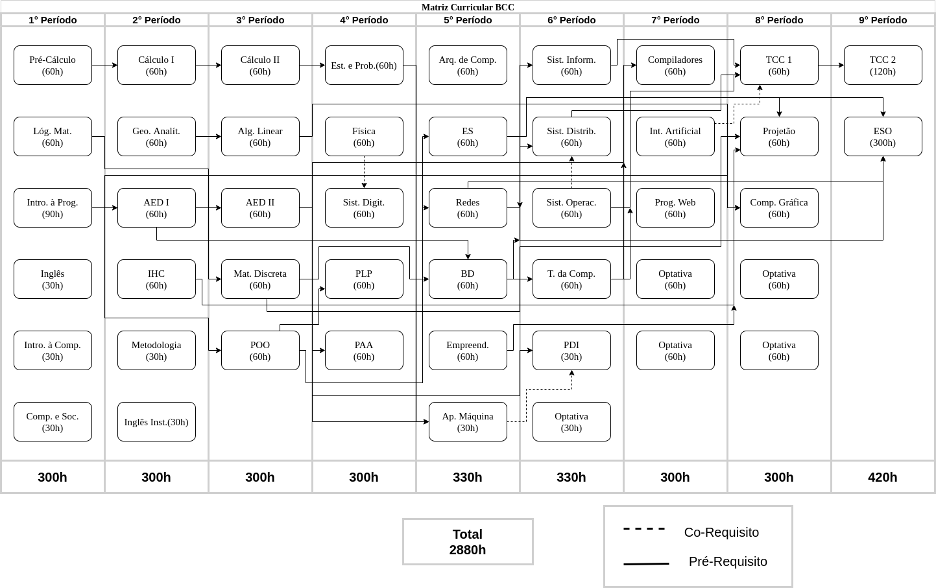
\includegraphics[width=\textwidth]{images/matriz_curricular_v3.png}
\end{figure}

\section{Quadro de Equivalência}

Diante da necessidade de adequar o perfil curricular do curso de Bacharelado em Ciência da Computação, os alunos que ingressarão no Curso a partir do semestre letivo de 2021.1 deverão compulsoriamente seguir a nova Matriz Curricular. Já os alunos que ingressaram em períodos anteriores ao semestre supracitado poderão, desde que atendam aos critérios definidos pelo Colegiado de Coordenação Didática - CCD do Curso, optar por seguir a antiga matriz curricular ou fazer a transição para a nova, buscando a equivalência de disciplinas entre as duas matrizes, conforme se mostra os Quadros 8 e 9. 

\begin{center}
  
  \begin{tiny}
    \begin{longtable}{p{6.5cm}cp{6.5cm}c}
      \caption{\label{quadro:disciplinas-obrigatorias-equivalentes}Disciplinas Obrigatórias Equivalentes.}\\
    \toprule
    \textbf{Matriz Antiga} & \textbf{CH} & \textbf{Matriz Nova} & \textbf{CH}\\
    \midrule
    - & & PRÉ-CÁLCULO & 60 \\ \midrule
    CCMP3056 INTRODUÇÃO À COMPUTAÇÃO C & 30 & INTRODUÇÃO À CIÊNCIA DA COMPUTAÇÃO & 30 \\ \midrule
    CCMP3071 COMPUTADORES E SOCIEDADE  & 30 & COMPUTADORES E SOCIEDADE & 30 \\ \midrule
    LETR3020 INGLÊS & 30 & INGLÊS  & 30 \\ \midrule
    MATM3031 CÁLCULO PARA COMPUTAÇÃO I  & 60 & CÁLCULO I & 60 \\ \midrule
    CCMP3070 INTERAÇÃO HUMANO-COMPUTADOR  & 60 & INTERAÇÃO HUMANO COMPUTADOR & 60 \\ \midrule
    - & & INGLÊS INSTRUMENTAL & 30 \\ \midrule
    CCMP3006 ALGORITMOS E ESTRUTURA DE DADOS I  & 60 & ALGORITMOS E ESTRUTURA DE DADOS & 60 \\ \midrule
    MATM3032 CÁLCULO PARA COMPUTAÇÃO II  & 60 & CÁLCULO II & 60 \\ \midrule
    MATM3019 ÁLGEBRA LINEAR  & 60 & ÁLGEBRA LINEAR I & 60 \\ \midrule
    CCMP3059 MATEMÁTICA DISCRETA  & 60 & MATEMÁTICA DISCRETA PARA COMPUTAÇÃO & 60 \\ \midrule
    CCMP3066 BANCO DE DADOS I & 60 & BANCO DE DADOS & 60 \\ \midrule
    - & & APRENDIZAGEM DE MÁQUINA & 30 \\ \midrule
    - & & PROGRAMAÇÃO WEB & 60  \\ \midrule
    CCMP3043 RECONHECIMENTO DE PADRÕES  & 60 & PROCESSAMENTO DIGITAL DE IMAGENS & 30 \\ \midrule
    CCMP3069 PROJETO DE DESENVOLVIMENTO & 90 & PROJETO DE DESENVOLVIMENTO DE SOFTWARE & 60 \\
\bottomrule
\end{longtable}
\end{tiny}
\end{center}

É importante salientar que o estudante que optar em realizar o processo de migração de perfil curricular do curso, não poderá solicitar retorno para o perfil de origem (antigo). Como pode ser observado pelo quadro de equivalências entre componentes curriculares das diferentes matrizes, o aluno que migrar para o novo perfil curricular poderá aproveitar as disciplinas já cursadas, incluindo as disciplinas optativas de acordo com o Quadro 9 abaixo.

\begin{center}
  
  \begin{tiny}
    \begin{longtable}{p{2cm}p{5.4cm}cp{5.4cm}c}
      \caption{\label{quadro:disciplinas-optativas-equivalentes}Disciplinas Optativas Equivalentes.}\\
    \toprule
    \textbf{Área} & \textbf{Matriz Antiga} & \textbf{CH} & \textbf{Matriz Nova} & \textbf{CH}\\
    \midrule
  Banco de Dados & - & & ADMINISTRAÇÃO DE BANCO DE DADOS & 60 \\ \cline{2-5}
    & CCMP3091 INTEGRAÇÃO DE DADOS E DATA WAREHOUSE & 60 & INTEGRAÇÃO DE DADOS E DATA WAREHOUSE & 60 \\ \cline{2-5}
    & - & & MINERAÇÃO DE DADOS & 60 \\ \cline{2-5}
    & - & & MODELAGEM CONCEITUAL DE DADOS & 60 \\ \cline{2-5}
    & - & & SISTEMAS DE INFORMAÇÃO GEOGRÁFICAS & 60 \\ \cline{2-5}
    & UAG00169 TÓPICOS ESPECIAIS EM BANCO DE DADOS & 60 & TÓPICOS ESPECIAIS EM BANCO DE DADOS & 60 \\ \midrule
  Engenharia da Computação & UAG00304 AVALIAÇÃO DE DESEMPENHO DE SISTEMAS & 60 & AVALIAÇÃO DE DESEMPENHO DE SISTEMAS & 60 \\ \cline{2-5}
    & - & & PROJETO DE SISTEMAS EMBARCADOS & 60 \\ \cline{2-5}
    & UAG00043 PROTOTIPAÇÃO DE CIRCUITOS DIGITAIS & 60 & PROTOTIPAÇÃO DE CIRCUITOS DIGITAIS & 60 \\ \cline{2-5}
    & - & & SISTEMAS DE TEMPO REAL & 60 \\ \midrule
  Engenharia de Software & CCMP3078 DESENVOLVIMENTO DE APLICAÇÕES MÓVEIS & 60 & DESENVOLVIMENTO DE APLICAÇÕES MÓVEIS & 60 \\ \cline{2-5}
  & CCMP3051 DESENVOLVIMENTO DISTRIBUÍDO DE SOFTWARE & 60 & DESENVOLVIMENTO DISTRIBUÍDO DE SOFTWARE & 60 \\ \cline{2-5}
    & - & & ESTIMATIVAS E MEDIÇÃO DE SOFTWARE & 60 \\ \cline{2-5}
    & - & & METODOLOGIAS ÁGEIS & 60 \\ \cline{2-5}
    & - & & PROGRAMAÇÃO ORIENTADA A ASPECTOS & 60 \\ \cline{2-5}
    & - & & PROGRAMAÇÃO ORIENTADA A OBJETOS II & 60 \\ \cline{2-5}
    & UAG00031 TESTE DE SOFTWARE & 60 & TESTE DE SOFTWARE & 60 \\ \cline{2-5}
    & - & & ESPECIFICAÇÃO FORMAL DE SOFTWARE & 60 \\ \cline{2-5}
    & - & & PROGRAMAÇÃO COMPETITIVA & 60 \\ \cline{2-5}
    & CCMP3080 TÓPICOS ESPECIAIS EM ENGENHARIA DE SOFTWARE & 60 & TÓPICOS ESPECIAIS EM ENGENHARIA DE SOFTWARE & 60 \\ \midrule
  Inteligência Computacional & - & & ALGORITMOS DE APRENDIZAGEM DE MÁQUINA & 60 \\ \cline{2-5}
    & - & & MÁQUINA DE VETORES DE SUPORTE & 60 \\ \cline{2-5}
    & - & & PROJETO EM APRENDIZAGEM DE MÁQUINA & 60 \\ \cline{2-5}
    & UAG00012 RECONHECIMENTO DE PADRÕES II & 60 & RECONHECIMENTO DE PADRÕES & 60 \\ \cline{2-5}
    & - & & REDUÇÃO DE DIMENSIONALIDADE EM APRENDIZAGEM DE MÁQUINA & 60 \\ \cline{2-5}
    & CCMP3086 TÓPICOS ESPECIAIS EM INTELIGÊNCIA ARTIFICIAL & 60 & TÓPICOS ESPECIAIS EM INTELIGÊNCIA ARTIFICIAL & 60 \\ \cline{2-5}
    & CCMP3039 REDES NEURAIS & 60 & REDES NEURAIS ARTIFICIAIS & 60 \\ \cline{2-5}
    & UAG00011 VISÃO COMPUTACIONAL & 60 & VISÃO COMPUTACIONAL & 60 \\ \midrule
  Matemática e Computação Teórica & - & & ÁLGEBRA LINEAR II & 60 \\ \cline{2-5}
    & - & & CÁLCULO III & 60 \\ \cline{2-5}
    & MATM3007 CÁLCULO PARA COMPUTAÇÃO III & 60 & CÁLCULO IV & 60 \\ \cline{2-5}
    & - & & CÁLCULO LAMBDA & 60 \\ \cline{2-5}
    & - & & INTRODUÇÃO À COMPUTAÇÃO QUÂNTICA  & 60 \\ \cline{2-5}
    & - & & OTIMIZAÇÃO COMBINATÓRIA (META-HEURÍSTICAS) & 60 \\ \cline{2-5}
    & - & & PESQUISA OPERACIONAL & 60 \\ \cline{2-5}
    & - & & REDES COMPLEXAS & 60 \\ \cline{2-5}
    & - & & TÓPICOS ESPECIAIS EM ALGORITMOS & 60 \\ \cline{2-5}
    & - & & TEORIA DOS NÚMEROS E CRIPTOGRAFIA & 60 \\ \cline{2-5}
    & - & & CRIPTOGRAFIA APLICADA & 60 \\ \cline{2-5}
    & MATM3017 CÁLCULO NUMÉRICO E COMPUTACIONAL & 60 & CÁLCULO NUMÉRICO E COMPUTACIONAL & 60 \\ \cline{2-5}
    & - & & ÁLGEBRA LINEAR COMPUTACIONAL & 60 \\ \cline{2-5}
    & - & & TÓPICOS MODELAGEM MATEMÁTICA CONTINUA & 60 \\ \midrule
  Mídia e Interação & - & & REALIDADE VIRTUAL E AUMENTADA & 60 \\ \cline{2-5}
    & CCMP3076 TÓPICOS ESPECIAIS EM PROCESSAMENTO DE SINAIS & 60 & TÓPICOS ESPECIAIS EM PROCESSAMENTO DE SINAIS & 60 \\ \cline{2-5}
    & CCMP3088 TÓPICOS ESPECIAIS EM MÍDIA E INTERAÇÃO & 60 & TÓPICOS ESPECIAIS EM MÍDIA E INTERAÇÃO & 60 \\ \midrule
  Redes e Sistemas Distribuídos & CCMP3085 GERENCIAMENTO DE REDES & 60 & GERENCIAMENTO DE REDES DE COMPUTADORES & 60 \\ \cline{2-5}
    & - & & INFRAESTRUTURA DE REDES E CABEAMENTO ESTRUTURADO & 60  \\ \cline{2-5}
    & - & & PROGRAMAÇÃO PARALELA E DISTRIBUÍDA & 60 \\ \cline{2-5}
    & - & & TÓPICOS ESPECIAIS EM REDES DE COMPUTADORES E SISTEMAS DISTRIBUÍDOS & 60 \\ \cline{2-5}
    & CCMP3079 SEGURANÇA DE REDES DE COMPUTADORES & 60 & SEGURANÇA DE REDES DE COMPUTADORES & 60 \\ \cline{2-5}
    & UAG00170 MODELAGEM DE DEPENDABILIDADE DE SISTEMAS COMPUTACIONAIS & 60 & MODELAGEM DE DEPENDABILIDADE & 60  \\ \midrule
  Tecnologia Educacional & EDUC3079 PROJETOS DE SISTEMAS EDUCACIONAIS & 60 & DESENVOLVIMENTO DE SOFTWARE EDUCACIONAL & 60 \\ \cline{2-5}
    & EDUC3048 INFORMÁTICA NA EDUCAÇÃO & 60 & INFORMÁTICA NA EDUCAÇÃO & 60 \\ \cline{2-5}
    & - & & TECNOLOGIAS ASSISTIVAS & 60 \\ \cline{2-5}
    & - & & TECNOLOGIAS, COGNIÇÃO E APRENDIZAGEM & 60 \\ \midrule
  Tecnologias da Informação & UAG00080 GESTÃO DA TECNOLOGIA DA INFORMAÇÃO & 60 & GESTÃO DA TECNOLOGIA DA INFORMAÇÃO & 60 \\ \cline{2-5}
    & CCMP3077 GESTÃO DE SERVIÇOS EM TI & 60 & GESTÃO DE SERVIÇOS EM TI & 60 \\ \cline{2-5}
    & UAG00079 GOVERNANÇA EM TECNOLOGIA DA INFORMAÇÃO & 60 & GOVERNANÇA EM TECNOLOGIA DA INFORMAÇÃO & 60 \\ \cline{2-5}
    & CCMP3083 TÓPICOS ESPECIAIS EM GESTÃO DE PROJETOS & 60 & TÓPICOS ESPECIAIS EM GESTÃO DE PROJETOS & 60 \\ \cline{2-5}
    & UAG00300 FUNDAMENTOS EM CIÊNCIA DE DADOS & 60 & FUNDAMENTOS EM CIÊNCIA DE DADOS & 60 \\ \cline{2-5}
    & UAG00024 GESTÃO DE PROCESSOS DE NEGÓCIO & 60 & GESTÃO DE PROCESSOS DE NEGÓCIO & 60 \\ \midrule
  - & EDUC3090 LÍNGUA BRASILEIRA DE SINAIS - LIBRAS L & 45 & LÍNGUA BRASILEIRA DE SINAIS - LIBRAS & 45 \\ 
\bottomrule
\end{longtable}
\end{tiny}
\end{center}

Também é importante destacar que, no momento da escolha de migração do Perfil Curricular, o discente aproveitará as Cargas Horárias oriundas de disciplinas que não apresentarem equivalência, serão contabilizadas para o Grupo de Componentes Optativos Livres.